% 20180521: Version for presentation at ECB 
% 20180330: Version for presentation at GMU after Jackie presents MESA 
% !TeX spellcheck = en_GB
\documentclass[11ptt]{beamer}
\beamerdefaultoverlayspecification{<+->}
%	\usetheme{warsaw}
\usepackage{moreverb}
\usepackage{setspace}
\usepackage{graphicx} %draft option suppresses graphics dvi display
\newcommand{\Prob}{\operatorname{Prob}}
\clubpenalty 5000
\widowpenalty 5000
\renewcommand{\baselinestretch}{1.23}
\usepackage{amsmath}
\usepackage{amsthm}
\usepackage{amsfonts}
\usepackage{amssymb}
\usepackage{bbm}
\usepackage{cancel}
% \newcommand{\E}{\mathbb{E}}
% \newcommand{\R}{\mathbb{R}}
% \newcommand{\pd}[2]{\frac{\partial#1}{\partial#2}}
\newcommand{\bi}{\begin{itemize}}
\newcommand{\ei}{\end{itemize}}
% \newcommand{\Die}{\mathsf{D}}
% \newcommand{\Live}{\cancel{\Die}}

\usepackage{ifthen}
\usepackage{econtexShortcuts}%\usepackage{econtexSetup}

\provideboolean{GMU}
\setboolean{GMU}{true}
\setboolean{GMU}{false}
\providecommand{\GMUYN}{\ifthenelse{\boolean{GMU}}}

\provideboolean{ECB}
\setboolean{ECB}{true}
\setboolean{ECB}{false}
\providecommand{\ECBYN}{\ifthenelse{\boolean{ECB}}}

\provideboolean{Elt}
\setboolean{Elt}{true}
\setboolean{Elt}{false}
\providecommand{\EltYN}{\ifthenelse{\boolean{Elt}}}

\provideboolean{SAFE}
\setboolean{SAFE}{true}
% \setboolean{SAFE}{false}
\providecommand{\SAFEYN}{\ifthenelse{\boolean{SAFE}}}

\providecommand{\ECBHideBegin}{\ifthenelse{\boolean{ECB}}{\setboolean{includeTF}{false}}{}}
\providecommand{\ECBHideEnd}{  \ifthenelse{\boolean{ECB}}{\setboolean{includeTF}{true}}{}}

\providecommand{\EltHideBegin}{\ifthenelse{\boolean{Elt}}{\setboolean{includeTF}{false}}{}}
\providecommand{\EltHideEnd}{  \ifthenelse{\boolean{Elt}}{\setboolean{includeTF}{true}}{}}

\providecommand{\SAFEHideBegin}{\ifthenelse{\boolean{SAFE}}{\setboolean{includeTF}{false}}{}}
\providecommand{\SAFEHideEnd}{  \ifthenelse{\boolean{SAFE}}{\setboolean{includeTF}{true}}{}}


\provideboolean{includeFrameTF}\setboolean{includeFrameTF}{true} % Default is to include 
\provideboolean{includeTextTF}\setboolean{includeTextTF}{true} % 
\provideboolean{includeTF}\setboolean{includeTF}{true} % 

\newcommand{\ifIncludeFrame}[1]{\ifthenelse{\boolean{includeFrameTF}}{#1}}
\newcommand{\ifIncludeText}[1]{\ifthenelse{\boolean{includeTextTF}}{#1}}
\newcommand{\ifInclude}[1]{\ifthenelse{\boolean{includeTF}}{#1}}

\author{Christopher Carroll, Matthew N. White, Jackie Kazil}

\title{An Introduction to the \\ Heterogeneous Agents Resources and toolKit}

\date{Generic Version, 2018-05-05} % Adapted by CDC from Intro-To-HARK_20180330_GMU.tex

\GMUYN{
  \date{Presentation at George Mason University \\ 2018-03-30}
}{}

\ECBYN{
  \author{Chris Carroll, Matt White}
  \date{Presentation at ECB \\ ``Workshop on Household Heterogeneity and Macroeconomics'' \\ 2018-05-22}

}{}

\EltYN{
  \author{Chris Carroll, Matt White}
  \date{Presentation at Bundesbank Conference \\ ``International Conference on Household Finance'' \\ 2018-05-24}
}{}


\SAFEYN{
  \author{Chris Carroll, Matt White}
  \date{Minicourse \\ ``Hands-On Heterogeneous Agent Macroeconomics'' \\ Goethe University and SAFE \\ 2018-05-28}
}{}

\usepackage{natbib}
\begin{document}

% ========== Intro slide =================
\begin{frame}
  \maketitle
\end{frame}

\ECBHideBegin\ifInclude{
\begin{frame}
  \frametitle{Agenda: A Flavor of HARK}
  \begin{enumerate}
  \item ``Microeconomic'' models in HARK: the \texttt{AgentType} class

  \item Example HARK model
    \begin{itemize}
    \item Consumption with permanent and transitory shocks to income
    \end{itemize}
    \SAFEHideBegin

    \ifInclude{
    \item Application: Structural estimation of parameters from MPC
    \begin{itemize}
    \item   \cite{fhnMPC}
    \end{itemize}}{}
  \SAFEHideEnd

  \item 30,000 foot view: What else is in HARK?
  \end{enumerate}
\end{frame}
}\ECBHideEnd

\begin{frame}
  \frametitle{Microeconomic Models in HARK}
  \begin{block}{}
    \bi
  \item Concern decision-making of one agent

  \item Discrete time

  \item Sequence of choices
    \begin{itemize}
    \item Household: Consumption, labor supply, portfolio choice, etc
    \item Firm: Investment, Employment, R\&D, ...
    \end{itemize}

  \item Agents treat inputs to problem as \textit{exogenous}
    \ei
  \end{block}
  % \ECBHideEnd

  \begin{block}{Key restriction: Essentially, Bellman equation}
    \begin{quote}Model solution can be constructed as iteration on sequence of ``one period problems,'' conditional on solution to subsequent period.
      \end{quote}
  \end{block}
\end{frame}

\ECBHideBegin\ifInclude{
  \begin{frame}
    \frametitle{Two kinds of heterogeneity}
      \bi
    \item \textit{Ex post} heterogeneity: Agents differ because a different sequence of events or shocks has happened to them
      \begin{itemize}
      \item Luck of the draw
      \end{itemize}

    \item \textit{Ex ante} heterogeneity: Agents differ in objectives, preferences, expectations, etc before anything ``happens'' to them
      \begin{itemize}
      \item Some people are more risk averse than others, e.g.
      \end{itemize}
      \ei

  \end{frame}
}{}\ECBHideEnd % 


%\GMUHideBegin\ifInclude{
  \begin{frame}    \frametitle{Crash Course in Object-Oriented Programming }
\centerline{\small (For more, see \href{http://github.com/econ-ark/HARK/Documentation/WhyPython.pdf}{WhyPython})}
    \begin{itemize}
    \item Traditional programming is \textit{procedural}:
      \begin{itemize}
      \item Accomplish task step by step; intuitive
      \end{itemize}
    \item Python is an \textit{object-oriented} language:

      \begin{itemize}
    \item[$\Rightarrow$] conceptual (and operational) groupings of similar things
        \item Start by defining needed items as a \textit{class}
      \begin{itemize}
      \item Example of a ``class'': \texttt{PerfForesightConsumerType}
      \end{itemize}
    \item \textbf{Attributes}: What characteristics define one \textit{instance}?
      \begin{itemize}
      \item e.g., an instance of a \texttt{PerfForesightConsumerType} with $\{\Rfree,\DiscFac,...\} = \{1.05,1/1.05, ...\}$ 
      \end{itemize}

    \item \textbf{Methods}: What actions can instances of the class ``do''?
      \begin{itemize}
        \item e.g., calculate `impatience' implied by its parameter values
        \end{itemize}

    \end{itemize}
  
\end{itemize}
  \end{frame}

  \ECBHideBegin
  \SAFEHideBegin

  \ifInclude{
  \begin{frame}
    \frametitle{Crash Course in Object-Oriented Programming (2/2)}

    \bi
  \item <1->Consider a class called \texttt{Jar}:
    \begin{itemize}
    \item A \texttt{Jar} is made of a \texttt{material}, has a \texttt{volume}, has \texttt{contents} (including names and volumes), and might be closed

    \item Methods: \texttt{open}, \texttt{close}, \texttt{addTo}, \texttt{dump}, \texttt{pourInto},... 
    \end{itemize}

  \item <2->And a class called \texttt{Can}:
    \begin{itemize}
    \item Just like \texttt{Jar}... but you can't \texttt{close} a \texttt{Can}
    \end{itemize}

  \item <2->Could have two classes with all those methods, but instead...

  \item <3->Make a class called \texttt{Container} with all those methods
    \begin{itemize}
    \item \texttt{Jar} is a subclass of \texttt{Container}, inherits its methods

    \item \texttt{Can} also a subclass, but overwrites \texttt{close} to do nothing
    \end{itemize}

    \ei



  \end{frame}
  }{}\ECBHideEnd\SAFEHideEnd
%}{}\GMUHideEnd


\begin{frame}
  \frametitle{HARK's ``Master Class'': \texttt{AgentType}}
  \bi
\item General purpose class for representing economic agents
\pause
\item Each model creates a subclass of \texttt{AgentType}
  \bi
  \item e.g. \texttt{PerfForesightConsumerType} is an \texttt{AgentType} subclass 
  \item Includes attributes, functions, and methods...
    \begin{itemize}
\item All \texttt{AgentType} subclasses have a \texttt{solve()} method
    \end{itemize}
    
  \ei
  \bi
%\item Just a universal backward induction loop...
\item Common structure $\Rightarrow$  different models ``play nicely'' together
\item Even though guts of \texttt{solve()} method differ for each subclass
\item Much easier to compare and exchange models
  \ei
\item Complex models extend basic ones through ``class inheritance''
  \ei
\end{frame}




\ECBHideBegin
% ========= What defines an agent's problem? 1 ========

\ifInclude{
\begin{frame}
  \frametitle{Defining An Agent's Problem}
  \bi
\item Define Behavior in some ``Terminal Period''
  
  \begin{itemize}
  \item Created by the class's method \texttt{solveTerminal}
    \item Example that can be used for finite or infinite horizon:
  \bi
\item \texttt{solution\_terminal.cFunc = consume everything}

\item \texttt{solution\_terminal.vPfunc = u'(consume everything)}
  \ei
    
  \end{itemize}
  

  
\item Define Information needed to solve one period back
  \begin{itemize}
  \item Variables, Distributions, Parameters, ...
  \end{itemize}

\item Keep Going ...
  \begin{itemize}
  \item Life Cycle? To birth
  \item Infinite Horizon? To convergence
  \item Infinite Horizon with Seasons? To seasonal convergence
    \item ...
  \end{itemize}
  
%  \pause
%\item <1->Are those things the same in every period, or do they vary across periods?
\SAFEYN{}{
\item Life Cycle consumption-saving model:
  \bi
\item \texttt{time\_inv = ['CRRA', 'Rfree', 'DiscFac', 'BoroCnstArt', 'vFuncBool', 'CubicBool', 'aXtraGrid']}

\item \texttt{time\_vary = ['IncomeDstn','LivPrb','PermGroFac']}
  \ei
  }{}
  \ei
\end{frame}
}{} % Defining an agent's problem (1/5)

\ifInclude{
% ========= What defines an agent's problem? 2 ========
\begin{frame}
  \frametitle{Defining An Agent's Problem}
  \bi
%\item Must know what values those variables, distributions, information have in each period

  \SAFEHideBegin
  \ifInclude{
\item What is the sequence of periods that agent will encounter?
  \begin{itemize}
  \item Life Cycle?
  \item Infinite Horizon?
  \item Infinite Horizon with Seasons?
    \item ...
    \end{itemize}
    }{}

  \SAFEHideEnd
  
\item Example: \texttt{IndShockConsumerType} consumption model:
  \bi
\item \texttt{CRRA = 3.2}

\item \texttt{DiscFac = 0.96}

\item \texttt{Rfree = 1.03}

\item \texttt{IncomeDstn = [too much to put here]}

  \item Life Cycle version:
  \begin{itemize}
    
\item \texttt{PermGroFac = [1.005,...,1.005,0.4,0.998,...,0.998]}

\item \texttt{LivPrb = [1,...,1,0.997,0.994,0.991,...,0]}
  \end{itemize}

  \item Infinite Horizon version:
  \begin{itemize}
    
\item \texttt{PermGroFac = [1.02]}

\item \texttt{LivPrb = [0.98]}
  \end{itemize}

  \ei
  \ei
\end{frame}
}

\SAFEHideBegin

\ifInclude{

  % ========= What defines an agent's problem? 3 ========
\begin{frame}
  \frametitle{Defining An Agent's Problem (3/5)}
  \bi
\item <1->How many times does that sequence of periods happen?

\item <1->Just once?  Ten times?  Indefinitely?
  \bi
\item \texttt{cycles = 1} : Sequence happens once, lifecycle model

\item \texttt{cycles = 40} : Sequence occurs 40 times in a loop

\item \texttt{cycles = 0} : Sequence repeats forever, infinite horizon
  \ei
  \ei
\end{frame}

}{}

\ifInclude{
  % ========= What defines an agent's problem? 4 ========
\begin{frame}
  \frametitle{Defining An Agent's Problem (4/5)}
  \bi
\item <1->Must know \textit{how} to solve a one period problem...

\item <1->...\textit{conditional} on solution to next period's problem...

\item <1->...given values of time (in)variant parameters

\item <2->Basic consumption-saving model:
  \bi
\item \texttt{solveOnePeriod = solveConsIndShock}

\item Inputs are named in \texttt{time\_vary} and \texttt{time\_inv}...

\item ...plus \texttt{solution\_next}, the output from previous call

\item Attributes of \texttt{solution\_next}: \texttt{cFunc}, \texttt{vPfunc}, \texttt{vPPfunc}, etc 
  \ei
  \ei
\end{frame}
}{}


\ifInclude{
% ========= What defines an agent's problem? 5========
\begin{frame}
  \frametitle{Defining An Agent's Problem}

  How does the backward induction loop start?
  \bi
\item Finite horizon: Need a terminal period solution or scrap value

\item Infinite horizon: Need an initial ``guess'' of the solution

\item \texttt{solution\_terminal} often can be found in closed form

\item Created by class method \texttt{solveTerminal}

\item Default consumption-saving problem:
  \bi
\item \texttt{solution\_terminal.cFunc = consume everything}

\item \texttt{solution\_terminal.vPfunc = u'(consume everything)}
  \ei
  \ei
\end{frame}
}{} % End of defining an agent's problem
\SAFEHideEnd

\ECBHideEnd

% ========== Example: consumption-saving =================

\begin{frame}\label{ModelStatement}
  \frametitle{Workhorse: Buffer Stock Consumption Model}

  Class \texttt{IndShockConsumerType}
  \begin{itemize}
  \item Inherits attributes of \texttt{PerfForesightConsumerType}
    \begin{itemize}
    \item Geometric discounting $\beta$ per period

  \item One choice: How much to consume vs save

  \item CRRA utility from consumption

  \item Exogenous interest factor for asset returns


    \end{itemize}
    \item Adds assumptions about income uncertainy and constraints
      \begin{itemize}
      \item     Mathematical Details: \hyperlink{ModelMath}{\beamerbutton{Formal model}}
      \end{itemize}

  \end{itemize}


\end{frame}


\begin{frame}
  \frametitle{Buffer Stock Model Consumption Function}
  \begin{center}
    \includegraphics[scale=0.65]{IndShockcFunc.pdf}
  \end{center}
  \centerline{Horizontal Axis: ``Money''; Vertical Axis: ``Spending''}
\end{frame}


\SAFEHideBegin

\ifInclude{
% =========== Structure ==================
\begin{frame}
  \frametitle{Object-Oriented Solution Methods}
  \begin{itemize}
  \item Models in HARK build up from each other
    \begin{itemize}
  \item ``Parent'' models are special cases of ``child'' models
    \end{itemize}

  \item Solvers in HARK are objects that act (a lot) like functions

  \item Each model must have a solver specified ...
    \begin{itemize}
  \item Default is to inherit solution method from parent solver...
  \item ...and then add or change its methods as needed
    \end{itemize}

  \end{itemize}
\end{frame}
}{}
\SAFEHideEnd

\SAFEHideBegin
\ECBHideBegin
\ifInclude{
\begin{frame}
  \frametitle{Small Extension: Costly Borrowing}
  \begin{itemize}
  \item Suppose we want a small extension to basic model: interest rate when borrowing greater than interest rate when saving.

  \item \texttt{ConsKinkedRsolver} inherits from \texttt{ConsIndShockSolver}
  \end{itemize}

\end{frame}

\begin{frame}
  \frametitle{Small Extension: Costly Borrowing}
  \texttt{ConsKinkedRsolver} inherits from \texttt{ConsIndShockSolver}

  \begin{block}{Additions to \texttt{\_\_init\_\_} method:}
    \begin{itemize}
    \item Store new attributes \texttt{Rboro} and \texttt{Rsave}
    \end{itemize}
  \end{block}

  \begin{block}{Additions to \texttt{prepareToCalcEndOfPrdvP}:}
    \begin{itemize}
    \item Four lines to use correct value of $R$ for each value of $a_t$

    \item One line to apply that change to calculation of $m_{t+1}$

    \item Three lines to recalculate minimum MPC and human wealth
    \end{itemize}
  \end{block}
\end{frame}

\begin{frame}
  \frametitle{Small Extension: Costly Borrowing}
  \begin{center}
    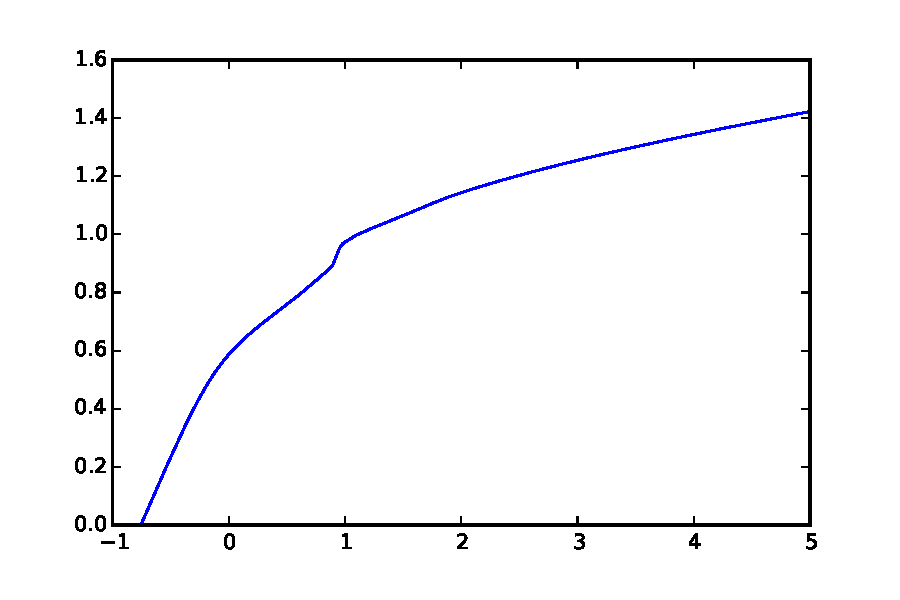
\includegraphics[scale=0.75]{KinkedRcFunc.pdf}
  \end{center}
\end{frame}
}{}\ECBHideEnd
\SAFEHideEnd

\ECBHideBegin
\SAFEHideBegin
\ifInclude{
% ============== Application: Fagereng et al ================
\begin{frame}
  \frametitle{An Application: Fagereng et al, Table 9}

  \begin{itemize}
  \item Fagereng et al report on household's consumption response to lottery winnings by quartile of prize size and deposits

  \item MPC universally declines with prize size and liquidity

  \item Is Table 9 consistent with a single-asset consumption-saving model?  How do we answer this in HARK?

  \end{itemize}
\end{frame}



\begin{frame}
  \frametitle{An Application: Fagereng et al, Table 9}

  Import HARK tools, model, and parameters\\
  (Importing basic packages omitted here)
  \begin{center}
    \includegraphics[trim = {0 0 0 8cm},scale=0.5,clip]{FagerengCode1.png}
  \end{center}

\end{frame}



\begin{frame}
  \frametitle{An Application: Fagereng et al, Table 9}

  Specify estimation parameters, MPC targets, and prize sizes
  \begin{center}
    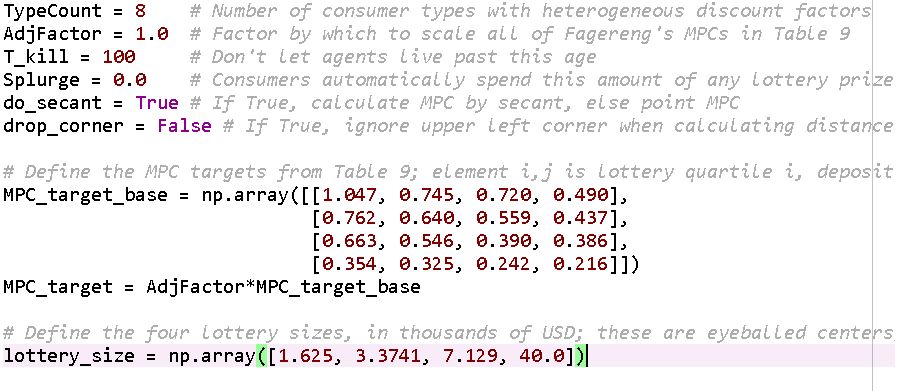
\includegraphics[scale=0.5]{FagerengCode2.png}
  \end{center}

\end{frame}



\begin{frame}
  \frametitle{An Application: Fagereng et al, Table 9}

  Modify parameters, make list of consumer types for estimation
  \begin{center}
    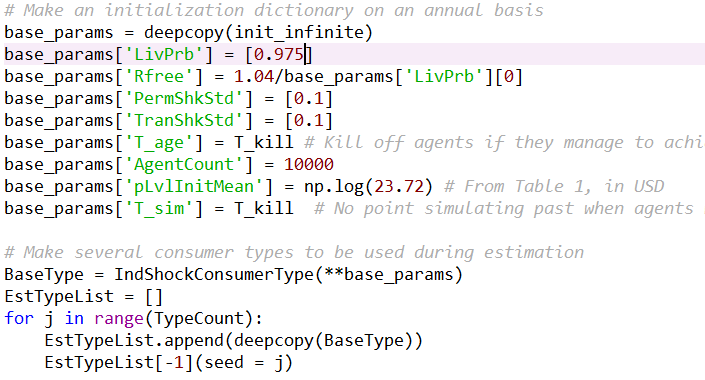
\includegraphics[scale=0.5]{FagerengCode3.png}
  \end{center}

\end{frame}



\begin{frame}
  \frametitle{An Application: Fagereng et al, Table 9}

  Objective function docstring
  \begin{center}
    \includegraphics[scale=0.5]{FagerengCodeDocString.png}
  \end{center}

\end{frame}



\begin{frame}
  \frametitle{An Application: Fagereng et al, Table 9}

  Distribute $\beta$ to consumers; solve and simulate; mark quartiles
  \includegraphics[scale=0.5]{FagerengCode4.png}

\end{frame}



\begin{frame}
  \frametitle{An Application: Fagereng et al, Table 9}

  Make nested list of MPCs by prize size and deposit quartiles
  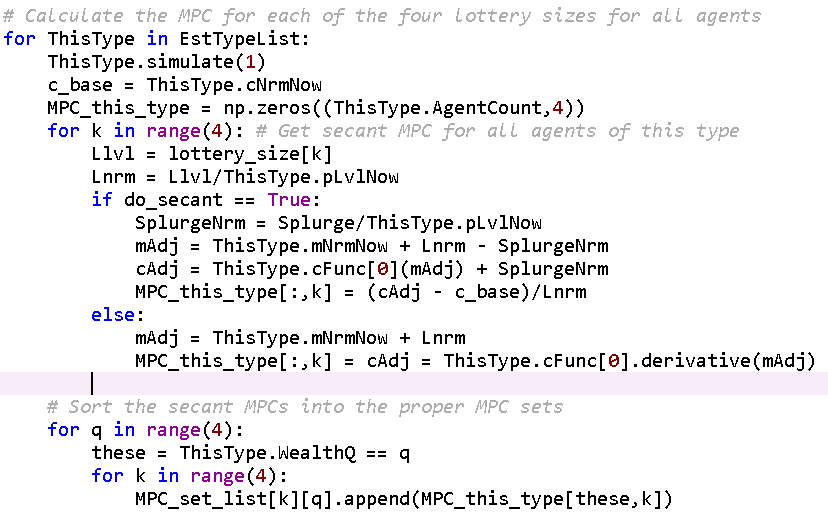
\includegraphics[scale=0.5]{FagerengCode5.png}


\end{frame}



\begin{frame}
  \frametitle{An Application: Fagereng et al, Table 9}

  Make simulated MPC table, calculate distance from targets
  \begin{center}
    \includegraphics[scale=0.5]{FagerengCode6.png}
  \end{center}

\end{frame}



\begin{frame}
  \frametitle{An Application: Fagereng et al, Table 9}

  Estimation and reporting

  \begin{center}
    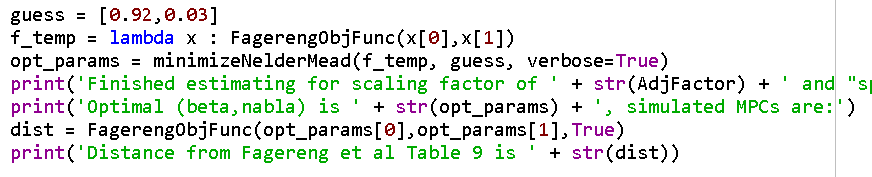
\includegraphics[scale=0.5]{FagerengCode7.png}
  \end{center}

\end{frame}
}{} % End of Fagering application
\ECBHideEnd
\SAFEHideEnd



% ========== Other models in HARK =================

\begin{frame}
  \frametitle{What Else Is In HARK or the Econ-ARK?}

  \begin{itemize}
  \item General purpose tools for generating and representing distributions, interpolated functions, etc

  \item Tools for estimation / optimization (fairly sparse)

  \item Framework for ``macroeconomic'' models: \texttt{Market} class

  \item Several extensions of basic consumption-saving model

  \item Some small demonstration exercises

  \item All results from several papers:
\begin{itemize}
  \item ''The Distribution of Wealth and the Marginal Propensity to Consume'' by \cite{cstwMPC}

  \item ''Sticky Expectations and Consumption Dynamics'' by \cite{cAndCwithStickyE}

    \item Several others are close
  \end{itemize}
  
    
  \item Much room for improvement: endogenous labor supply (e.g.)

  \end{itemize}

\end{frame}



\begin{frame}
  \frametitle{Other Consumption-Saving Models in HARK}
  \begin{itemize}
  \item <1->\texttt{TractableBufferStock}: Highly specialized idiosync shocks

  \item <2->\texttt{MarkovModel}: $\PLives,\Gamma,F_\theta,F_\psi,R$ vary by discrete state

  \item <3->\texttt{ExplicitPermInc}: Same as \texttt{IndShock}, but not normalized

  \item <3->\texttt{PersistentShock}: ``Permanent'' shocks not fully permanent

  \item <4->\texttt{MedShock}: 2nd cons good with random marginal utility

  \item <5->\texttt{MedHealthShock}:* Medical shocks plus discrete health states

  \item <5->\texttt{DynInsSel}:* ...plus choice over medical insurance contracts
  \end{itemize}
  And even more to come...
\end{frame}


\begin{frame}
  \frametitle{Consumption-Saving Model Tree}
  \begin{center}
    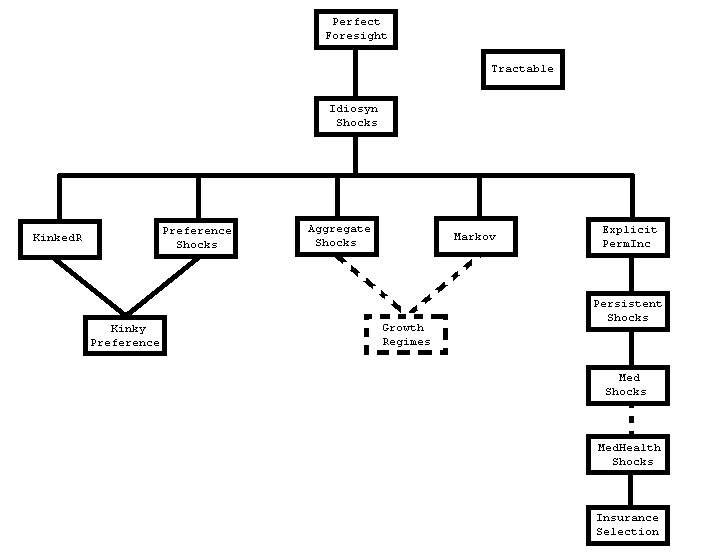
\includegraphics[scale=0.5]{NamesModelTree.png}
  \end{center}
\end{frame}

% 20180317: No changes until here
% =========== Expanded model tree? ==================

\begin{frame}\label{DiscussionTopics}
  \frametitle{Topics for Further Discussion}

  Time is short, but I could talk about...
  \begin{itemize}
  \item Class inheritance / model recombination \hyperlink{Recombination}{\beamerbutton{Link}}

  \item ``Macroeconomic'' framework and models \hyperlink{Macroeconomics}{\beamerbutton{Link}}

  \item To do: endogenous labor supply models  \hyperlink{LaborSupply}{\beamerbutton{Link}}

  \item To do: durable goods models \hyperlink{DurableGoods}{\beamerbutton{Link}}

  \item To do: various bits, large and small \hyperlink{StructuralChanges}{\beamerbutton{Link}}
  \end{itemize}
\end{frame}


\begin{frame}\label{DiscussionTopics}
  \frametitle{Topics for Further Discussion}

  Time is short, but I could talk about...
  \begin{itemize}
  \item Class inheritance / model recombination \hyperlink{Recombination}{\beamerbutton{Link}}

  \item ``Macroeconomic'' framework and models \hyperlink{Macroeconomics}{\beamerbutton{Link}}

  \item Roadmap \hyperlink{HARKFuture}{\beamerbutton{Link}}
  \end{itemize}
\end{frame}

\begin{verbatimwrite}{../../Roadmaps/HARK/Intro-To-HARK-From.tex}
  \begin{frame}\label{HARKFuture}\frametitle{Planned Future of Additions to HARK}

    \begin{enumerate}
    \item Endogenous labor supply models  \hyperlink{LaborSupply}{\beamerbutton{Link}}
    \item Durable goods models \hyperlink{DurableGoods}{\beamerbutton{Link}}
    \item Various bits, large and small \hyperlink{StructuralChanges}{\beamerbutton{Link}}
    \end{enumerate}
  \end{frame}

  % ==================== LABOR SUPPLY MODELS ===============

  \begin{frame}\label{LaborSupply}
    \frametitle{The Future of HARK: Incorporating Labor (1/4)}
    Model of labor supply on intensive margin:
    \begin{equation*}
      u(c,\ell) = ((1-\ell)^\alpha c)^{1-\rho}/(1-\rho),
    \end{equation*}
    \begin{equation*}
      v_t(b_t,\theta_t) = \max_{c_t, \ell_t} u(c_t,\ell_t) + \beta \PLives_t \Ex_t \left[(\psi_{t+1} \Gamma_t)^{1-\rho} v_{t+1}(b_{t+1},\theta_{t+1}) \right] \text{ s.t. }
    \end{equation*}
    \begin{equation*}
      y_t = \ell_t \theta_t, \qquad \ell_t \in [0,1],
    \end{equation*}
    \begin{equation*}
      a_t = m_t + y_t - c_t, \hspace{0.5cm} a_t \geq \underline{a},
    \end{equation*}
    \begin{equation*}
      b_{t+1} = R/(\Gamma_t \psi_{t+1}) a_t, 
    \end{equation*}
    \begin{equation*}
      \psi_{t+1} \sim F_{\psi t+1}(\psi), \hspace{0.5cm} \theta_{t+1} \sim F_{\theta t+1}(\theta), \hspace{0.25cm} \Ex[\psi_{t+1}] = 1.
    \end{equation*}
  \end{frame}


  \begin{frame}
    \frametitle{The Future of HARK: Incorporating Labor (2/4)}
    Model of labor supply on extensive margin:
    \begin{equation*}
      u(c,\ell) = c^{1-\rho}/(1-\rho) - \alpha \ell,
    \end{equation*}
    \begin{equation*}
      v_t(b_t,\theta_t,\ell_{t-1}) = \max_{c_t, \ell_t} u(c_t,\ell_t) + \beta \PLives_t \Ex_t \left[(\psi_{t+1} \Gamma_t)^{1-\rho} v_{t+1}(b_{t+1},\theta_{t+1},\ell_t) \right] \text{ s.t. }
    \end{equation*}
    \begin{equation*}
      y_t = \ell_t \theta_t, \qquad \ell_t \in \{0,\ell_{t-1}\},
    \end{equation*}
    \begin{equation*}
      a_t = m_t + y_t - c_t, \hspace{0.5cm} a_t \geq \underline{a},
    \end{equation*}
    \begin{equation*}
      b_{t+1} = R/(\Gamma_t \psi_{t+1}) a_t, 
    \end{equation*}
    \begin{equation*}
      \psi_{t+1} \sim F_{\psi t+1}(\psi), \hspace{0.5cm} \theta_{t+1} \sim F_{\theta t+1}(\theta), \hspace{0.25cm} \Ex[\psi_{t+1}] = 1.
    \end{equation*}
  \end{frame}



  \begin{frame}
    \frametitle{The Future of HARK: Incorporating Labor (3/4)}
    Model of endogenous employment search:
    \begin{equation*}
      u(c,s) = ((1-s)^\alpha c)^{1-\rho}/(1-\rho),
    \end{equation*}
    \begin{equation*}
      v_t(m_t,e_t) = \max_{c_t,s_t} u(c_t,s_t) + \beta \PLives_t \Ex_t \left[(\psi_{t+1} \Gamma_t)^{1-\rho} v_{t+1}(m_{t+1},e_{t+1}) \right] \text{ s.t. }
    \end{equation*}
    \begin{equation*}
      a_t = m_t - c_t, \hspace{0.5cm} a_t \geq \underline{a}, \hspace{0.5cm} s_t \in [0,1],
    \end{equation*}
    \begin{equation*}
      m_{t+1} = R/(\Gamma^e_t \psi_{t+1}) a_t + \theta_t e_{t+1} + \underline{b}(1-e_{t+1}), 
    \end{equation*}
    \begin{equation*}
      \Prob(e_{t+1} = 1 | e_t = 0) = s_t, \qquad \Prob(e_{t+1} = 0 | e_t = 1) = \mho,
    \end{equation*}
    \begin{equation*}
      \psi_{t+1} \sim F^e_{\psi t+1}(\psi), \hspace{0.5cm} \theta_{t+1} \sim F_{\theta t+1}(\theta), \hspace{0.25cm} \Ex[\psi_t] = 1.
    \end{equation*}
  \end{frame}



  \begin{frame}
    \frametitle{The Future of HARK: Incorporating Labor (4/4)}
    Applications of \texttt{Market} for labor models:
    \bi
  \item Non-trivial calculation of $L_t = \int_0^1 \ell_{it} p_{it} \theta_{it} di$ for Cobb-Douglas

  \item Disutility of employment search and probability of job loss depend on labor market slackness

  \item Can look at behavior in response to change in SS, etc
    \ei

    \hyperlink{DiscussionTopics}{\beamerbutton{Back}}
  \end{frame}

  % ===================== DURABLE GOODS =========================

  \begin{frame}\label{DurableGoods}
    \frametitle{The Future of HARK: Durable Goods (1/3)}

    General durable goods model:
    \begin{equation*}
      u(c,d) = (c^\alpha,d^{1-\alpha})^{1-\rho}/(1-\rho).
    \end{equation*}
    \begin{equation*}
      v_t(m_t,d_t) = \max_{c_t,i_t} u(c_t,d_t) + \beta \PLives_t \Ex_t \left[(\psi_{t+1} \Gamma_t)^{1-\rho} v_{t+1}(m_{t+1},d_{t+1}) \right] \text{ s.t. }
    \end{equation*}
    \begin{equation*}
      a_t = m_t - c_t, \hspace{0.5cm} a_t \geq \underline{a},
    \end{equation*}
    \begin{equation*}
      D_t = d_t + g(i_t), \hspace{0.5cm} d_{t+1} = (1-\delta_{t+1})D_t, \hspace{0.5cm} \delta_{t+1} \sim F_{\delta}(\delta),
    \end{equation*}
    \begin{equation*}
      m_{t+1} = R/(\Gamma_t \psi_{t+1}) a_t + \theta_{t+1}, 
    \end{equation*}
    \begin{equation*}
      \psi_{t+1} \sim F_{\psi t+1}(\psi), \hspace{0.5cm} \theta_{t+1} \sim F_{\theta t+1}(\theta), \hspace{0.25cm} \Ex[\psi_t] = 1.
    \end{equation*}
  \end{frame}



  \begin{frame}
    \frametitle{The Future of HARK: Durable Goods (2/3)}
    Variations of durable goods model require different solvers:
    \bi
  \item <1-> Easiest case: $g(i_t)$ is concave, $i_t \in \Rfree$.  Every end-of-period state $(a_t,D_t)$ associated with \textit{some} beginning of period state.

  \item <1->Slightly harder: $i_t \geq 0$, must handle constraint

  \item <2->Somewhat harder: $g(i_t) = \pi i_t$.  One locus in $(a_t,D_t)$ space is optimal; each point on optimal $(a_t,D_t)$ locus associated with locus in $(m_t,d_t)$ space.

  \item <3->Even harder: $g(i_t) = \widehat{g}(i_t) + K \mathbf{1}(i_t \neq 0)$, with $\widehat{g}(0) = 0$ and $\widehat{g}(\cdot)$ concave.  Must check $i_t=0$ soln everywhere, discont.

  \item <4->Just ugh: $g(i_t) = \pi i_t +K \mathbf{1}(i_t \neq 0)$, $i_t \geq 0$.
    \ei
  \end{frame}


  \begin{frame}
    \frametitle{The Future of HARK: Durable Goods (3/3)}
    Applications for \texttt{Market} with durable goods:
    \bi
  \item Endogenous pricing of durable good: housing market

  \item Dynamics of demand for durables after an aggregate shock

  \item Some specifications overlap with health models
    \ei

    \hyperlink{DiscussionTopics}{\beamerbutton{Back}}
  \end{frame}


  % ============= VARIOUS TO DO ITEMS ====================================

  \begin{frame}\label{StructuralChanges}
    \frametitle{The Future of HARK: Small To-Do Items}
    Contributions that would get your feet wet in HARK:
    \bi
  \item <1->Extend perfect foresight to handle borrowing constraint

  \item <1->Bequest motives: warm glow, other?

  \item <2->Fix/improve aggregate shocks model: handle life cycle models

  \item <2->Fix/generalize \texttt{ExplicitPermInc} models: \texttt{PermGroFunc}

  \item <2->Portfolio allocation models; eventually: asset pricing

  \item <3->Advanced features on more solvers: cubic spline interpolation

  \item <3->Various numeric methods detached from particular models
    \ei
  \end{frame}


  \begin{frame}
    \frametitle{The Future of HARK: Heavy Lifting}
    If you're feeling ambitious or are comfortable with HARK:
    \bi
  \item <1->Incorporate \texttt{opencl4py} with basic consumption-saving model.  ``Repack'' model inputs into memory buffers, pass to OpenCL solver.  OpenCL simulator: easier, big gains for some models.

  \item <2->Aggregate shocks with explicit permanent income.  One endogenous state variable, two exogenous state variables.  Future candidate for GPU computing.

  \item <3->Generalized Markov solver: make ``solution schema'' so that Markov state can be added to any correctly specified solver

  \item <4->Models of firm creation / bankruptcy / investment / hiring
    \ei

    \hyperlink{DiscussionTopics}{\beamerbutton{Back}}
  \end{frame}


\end{verbatimwrite}
  \begin{frame}\label{HARKFuture}\frametitle{Planned Future of Additions to HARK}

    \begin{enumerate}
    \item Endogenous labor supply models  \hyperlink{LaborSupply}{\beamerbutton{Link}}
    \item Durable goods models \hyperlink{DurableGoods}{\beamerbutton{Link}}
    \item Various bits, large and small \hyperlink{StructuralChanges}{\beamerbutton{Link}}
    \end{enumerate}
  \end{frame}

  % ==================== LABOR SUPPLY MODELS ===============

  \begin{frame}\label{LaborSupply}
    \frametitle{The Future of HARK: Incorporating Labor (1/4)}
    Model of labor supply on intensive margin:
    \begin{equation*}
      u(c,\ell) = ((1-\ell)^\alpha c)^{1-\rho}/(1-\rho),
    \end{equation*}
    \begin{equation*}
      v_t(b_t,\theta_t) = \max_{c_t, \ell_t} u(c_t,\ell_t) + \beta \PLives_t \Ex_t \left[(\psi_{t+1} \Gamma_t)^{1-\rho} v_{t+1}(b_{t+1},\theta_{t+1}) \right] \text{ s.t. }
    \end{equation*}
    \begin{equation*}
      y_t = \ell_t \theta_t, \qquad \ell_t \in [0,1],
    \end{equation*}
    \begin{equation*}
      a_t = m_t + y_t - c_t, \hspace{0.5cm} a_t \geq \underline{a},
    \end{equation*}
    \begin{equation*}
      b_{t+1} = R/(\Gamma_t \psi_{t+1}) a_t,
    \end{equation*}
    \begin{equation*}
      \psi_{t+1} \sim F_{\psi t+1}(\psi), \hspace{0.5cm} \theta_{t+1} \sim F_{\theta t+1}(\theta), \hspace{0.25cm} \Ex[\psi_{t+1}] = 1.
    \end{equation*}
  \end{frame}


  \begin{frame}
    \frametitle{The Future of HARK: Incorporating Labor (2/4)}
    Model of labor supply on extensive margin:
    \begin{equation*}
      u(c,\ell) = c^{1-\rho}/(1-\rho) - \alpha \ell,
    \end{equation*}
    \begin{equation*}
      v_t(b_t,\theta_t,\ell_{t-1}) = \max_{c_t, \ell_t} u(c_t,\ell_t) + \beta \PLives_t \Ex_t \left[(\psi_{t+1} \Gamma_t)^{1-\rho} v_{t+1}(b_{t+1},\theta_{t+1},\ell_t) \right] \text{ s.t. }
    \end{equation*}
    \begin{equation*}
      y_t = \ell_t \theta_t, \qquad \ell_t \in \{0,\ell_{t-1}\},
    \end{equation*}
    \begin{equation*}
      a_t = m_t + y_t - c_t, \hspace{0.5cm} a_t \geq \underline{a},
    \end{equation*}
    \begin{equation*}
      b_{t+1} = R/(\Gamma_t \psi_{t+1}) a_t,
    \end{equation*}
    \begin{equation*}
      \psi_{t+1} \sim F_{\psi t+1}(\psi), \hspace{0.5cm} \theta_{t+1} \sim F_{\theta t+1}(\theta), \hspace{0.25cm} \Ex[\psi_{t+1}] = 1.
    \end{equation*}
  \end{frame}



  \begin{frame}
    \frametitle{The Future of HARK: Incorporating Labor (3/4)}
    Model of endogenous employment search:
    \begin{equation*}
      u(c,s) = ((1-s)^\alpha c)^{1-\rho}/(1-\rho),
    \end{equation*}
    \begin{equation*}
      v_t(m_t,e_t) = \max_{c_t,s_t} u(c_t,s_t) + \beta \PLives_t \Ex_t \left[(\psi_{t+1} \Gamma_t)^{1-\rho} v_{t+1}(m_{t+1},e_{t+1}) \right] \text{ s.t. }
    \end{equation*}
    \begin{equation*}
      a_t = m_t - c_t, \hspace{0.5cm} a_t \geq \underline{a}, \hspace{0.5cm} s_t \in [0,1],
    \end{equation*}
    \begin{equation*}
      m_{t+1} = R/(\Gamma^e_t \psi_{t+1}) a_t + \theta_t e_{t+1} + \underline{b}(1-e_{t+1}),
    \end{equation*}
    \begin{equation*}
      \Prob(e_{t+1} = 1 | e_t = 0) = s_t, \qquad \Prob(e_{t+1} = 0 | e_t = 1) = \mho,
    \end{equation*}
    \begin{equation*}
      \psi_{t+1} \sim F^e_{\psi t+1}(\psi), \hspace{0.5cm} \theta_{t+1} \sim F_{\theta t+1}(\theta), \hspace{0.25cm} \Ex[\psi_t] = 1.
    \end{equation*}
  \end{frame}



  \begin{frame}
    \frametitle{The Future of HARK: Incorporating Labor (4/4)}
    Applications of \texttt{Market} for labor models:
    \bi
  \item Non-trivial calculation of $L_t = \int_0^1 \ell_{it} p_{it} \theta_{it} di$ for Cobb-Douglas

  \item Disutility of employment search and probability of job loss depend on labor market slackness

  \item Can look at behavior in response to change in SS, etc
    \ei

    \hyperlink{DiscussionTopics}{\beamerbutton{Back}}
  \end{frame}

  % ===================== DURABLE GOODS =========================

  \begin{frame}\label{DurableGoods}
    \frametitle{The Future of HARK: Durable Goods (1/3)}

    General durable goods model:
    \begin{equation*}
      u(c,d) = (c^\alpha,d^{1-\alpha})^{1-\rho}/(1-\rho).
    \end{equation*}
    \begin{equation*}
      v_t(m_t,d_t) = \max_{c_t,i_t} u(c_t,d_t) + \beta \PLives_t \Ex_t \left[(\psi_{t+1} \Gamma_t)^{1-\rho} v_{t+1}(m_{t+1},d_{t+1}) \right] \text{ s.t. }
    \end{equation*}
    \begin{equation*}
      a_t = m_t - c_t, \hspace{0.5cm} a_t \geq \underline{a},
    \end{equation*}
    \begin{equation*}
      D_t = d_t + g(i_t), \hspace{0.5cm} d_{t+1} = (1-\delta_{t+1})D_t, \hspace{0.5cm} \delta_{t+1} \sim F_{\delta}(\delta),
    \end{equation*}
    \begin{equation*}
      m_{t+1} = R/(\Gamma_t \psi_{t+1}) a_t + \theta_{t+1},
    \end{equation*}
    \begin{equation*}
      \psi_{t+1} \sim F_{\psi t+1}(\psi), \hspace{0.5cm} \theta_{t+1} \sim F_{\theta t+1}(\theta), \hspace{0.25cm} \Ex[\psi_t] = 1.
    \end{equation*}
  \end{frame}



  \begin{frame}
    \frametitle{The Future of HARK: Durable Goods (2/3)}
    Variations of durable goods model require different solvers:
    \bi
  \item <1-> Easiest case: $g(i_t)$ is concave, $i_t \in \Rfree$.  Every end-of-period state $(a_t,D_t)$ associated with \textit{some} beginning of period state.

  \item <1->Slightly harder: $i_t \geq 0$, must handle constraint

  \item <2->Somewhat harder: $g(i_t) = \pi i_t$.  One locus in $(a_t,D_t)$ space is optimal; each point on optimal $(a_t,D_t)$ locus associated with locus in $(m_t,d_t)$ space.

  \item <3->Even harder: $g(i_t) = \widehat{g}(i_t) + K \mathbf{1}(i_t \neq 0)$, with $\widehat{g}(0) = 0$ and $\widehat{g}(\cdot)$ concave.  Must check $i_t=0$ soln everywhere, discont.

  \item <4->Just ugh: $g(i_t) = \pi i_t +K \mathbf{1}(i_t \neq 0)$, $i_t \geq 0$.
    \ei
  \end{frame}


  \begin{frame}
    \frametitle{The Future of HARK: Durable Goods (3/3)}
    Applications for \texttt{Market} with durable goods:
    \bi
  \item Endogenous pricing of durable good: housing market

  \item Dynamics of demand for durables after an aggregate shock

  \item Some specifications overlap with health models
    \ei

    \hyperlink{DiscussionTopics}{\beamerbutton{Back}}
  \end{frame}


  % ============= VARIOUS TO DO ITEMS ====================================

  \begin{frame}\label{StructuralChanges}
    \frametitle{The Future of HARK: Small To-Do Items}
    Contributions that would get your feet wet in HARK:
    \bi
  \item <1->Extend perfect foresight to handle borrowing constraint

  \item <1->Bequest motives: warm glow, other?

  \item <2->Fix/improve aggregate shocks model: handle life cycle models

  \item <2->Fix/generalize \texttt{ExplicitPermInc} models: \texttt{PermGroFunc}

  \item <2->Portfolio allocation models; eventually: asset pricing

  \item <3->Advanced features on more solvers: cubic spline interpolation

  \item <3->Various numeric methods detached from particular models
    \ei
  \end{frame}


  \begin{frame}
    \frametitle{The Future of HARK: Heavy Lifting}
    If you're feeling ambitious or are comfortable with HARK:
    \bi
  \item <1->Incorporate \texttt{opencl4py} with basic consumption-saving model.  ``Repack'' model inputs into memory buffers, pass to OpenCL solver.  OpenCL simulator: easier, big gains for some models.

  \item <2->Aggregate shocks with explicit permanent income.  One endogenous state variable, two exogenous state variables.  Future candidate for GPU computing.

  \item <3->Generalized Markov solver: make ``solution schema'' so that Markov state can be added to any correctly specified solver

  \item <4->Models of firm creation / bankruptcy / investment / hiring
    \ei

    \hyperlink{DiscussionTopics}{\beamerbutton{Back}}
  \end{frame}




% ===================== Consumption-saving model math ================================================
\begin{frame}\label{ModelMath}
  \frametitle{Example Model: Basic Consumption-Saving}

  Consumption-saving model with idiosyncratic permanent and transitory shocks to income (normalized format):

  \begin{equation*}
    u(c) = c^{1-\rho}/(1-\rho).
  \end{equation*}
  \begin{equation*}
    v_t(m_t) = \max_{c_t} u(c_t) + \beta \PLives_t \Ex_t \left[(\psi_{t+1} \Gamma_{t+1})^{1-\rho} v_{t+1}(m_{t+1}) \right] \text{ s.t. }
  \end{equation*}
  \begin{equation*}
    a_t = m_t - c_t, \hspace{0.5cm} a_t \geq \underline{a},
  \end{equation*}
  \begin{equation*}
    m_{t+1} = R/(\Gamma_{t+1} \psi_{t+1}) a_t + \theta_{t+1}, 
  \end{equation*}
  \begin{equation*}
    \psi_{t+1} \sim F_{\psi t+1}(\psi), \hspace{0.5cm} \theta_{t+1} \sim F_{\theta t+1}(\theta), \hspace{0.25cm} \Ex[\psi_t] = 1.
  \end{equation*}
\end{frame}



\begin{frame}
  \frametitle{Example Model: Basic Consumption-Saving}

  Model solution in two lines:

  \begin{equation*}
    \text{FOC: } u'(c_t) = R \beta \PLives \Ex_t \left[(\psi_{t+1} \Gamma_{t+1})^{-\rho} v'_{t+1}(m_{t+1}) \right],
  \end{equation*}
  \begin{equation*}
    \text{EC: } v'_t(m_t) = u'(c_t).
  \end{equation*}

  Will use endogenous grid method:
  \begin{equation*}
    \mathfrak{v}'_t(a_t) \equiv R \beta \Ex_t \left[(\psi_{t+1} \Gamma_{t+1})^{-\rho} v'_{t+1}(m_{t+1}) | a_t\right],
  \end{equation*}
  \begin{equation*}
    c_t = \mathfrak{v}'_t(a_t)^{-\rho}, \hspace{0.5cm} m_t = a_t + c_t \text{ (for exogenous set of } \{a_t\} \text{)}.
  \end{equation*}

  \hyperlink{ModelStatement}{\beamerbutton{Back}}
\end{frame}





% ========== Kinked R ==========================================
\begin{frame}\label{Recombination}
  \frametitle{Consumption-Saving Model Tree}
  \begin{center}
    \includegraphics[scale=0.5]{TreeHighlight2.png}
  \end{center}
\end{frame}

\begin{frame}
  \frametitle{Consumption-Saving Model Tree}
  \begin{center}
    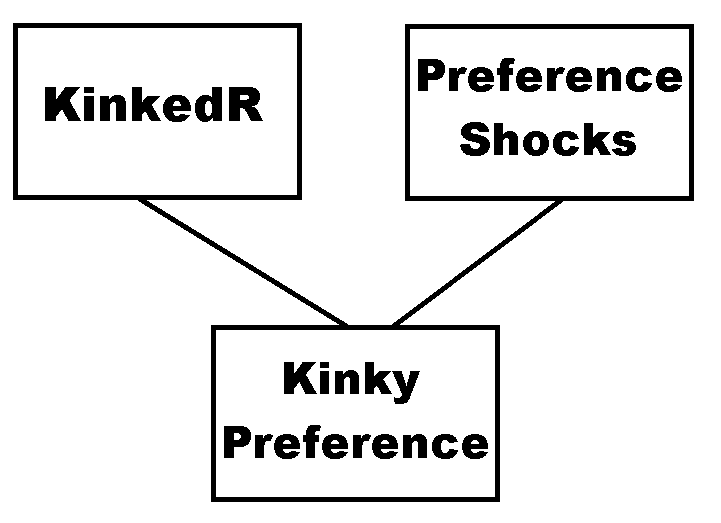
\includegraphics[scale=0.5]{TreeZoom2.png}
  \end{center}
\end{frame}


\begin{frame}
  \frametitle{Kinked R: Costly Borrowing (1/3)}
  Make one small adjustment to idiosyncratic income shocks model: interest rate on borrowing is higher than rate on saving.

  \begin{eqnarray*}
    u(c) &=& \frac{c^{1-\rho}}{1-\rho}, \\
    v(m_t) &=& \max_{c_t} u(c_t) + \beta \PLives_{t+1} \Ex [v_{t+1}(m_{t+1}) ], \\
    a_t &=& m_t - c_t, \qquad a_t \geq \underline{a}, \\
    m_{t+1} &=& R/(\Gamma_{t+1} \psi_{t+1}) a_t + \theta_{t+1}, \\
    \theta_{t+1} \sim F_{\theta t+1}, &\qquad& \psi_{t+1} \sim F_{\psi t+1}, \hspace{0.25cm} \Ex[\psi_{t+1}] = 1, \\
    R &=& \begin{cases}
      R_{boro} & \text{if  } a_t < 0 \\
      R_{save} & \text{if  } a_t > 0
    \end{cases}, \qquad R_{boro} \geq R_{save}.
  \end{eqnarray*}
\end{frame}


\begin{frame}
  \frametitle{Kinked R: Costly Borrowing (2/3)}
  \texttt{ConsKinkedRsolver} inherits from \texttt{ConsIndShockSolver}

  \begin{block}{Additions to \texttt{\_\_init\_\_} method:}
    \begin{itemize}
    \item Store new attributes \texttt{Rboro} and \texttt{Rsave}
    \end{itemize}
  \end{block}
  \begin{block}{Additions to \texttt{prepareToCalcEndOfPrdvP}:}
    \begin{itemize}
    \item Four lines to use correct value of $R$ for each value of $a_t$

    \item One line to apply that change to calculation of $m_{t+1}$

    \item Three lines to recalculate minimum MPC and human wealth
    \end{itemize}
  \end{block}
\end{frame}


\begin{frame}
  \frametitle{Kinked R: Costly Borrowing (3/3)}
  \begin{center}
    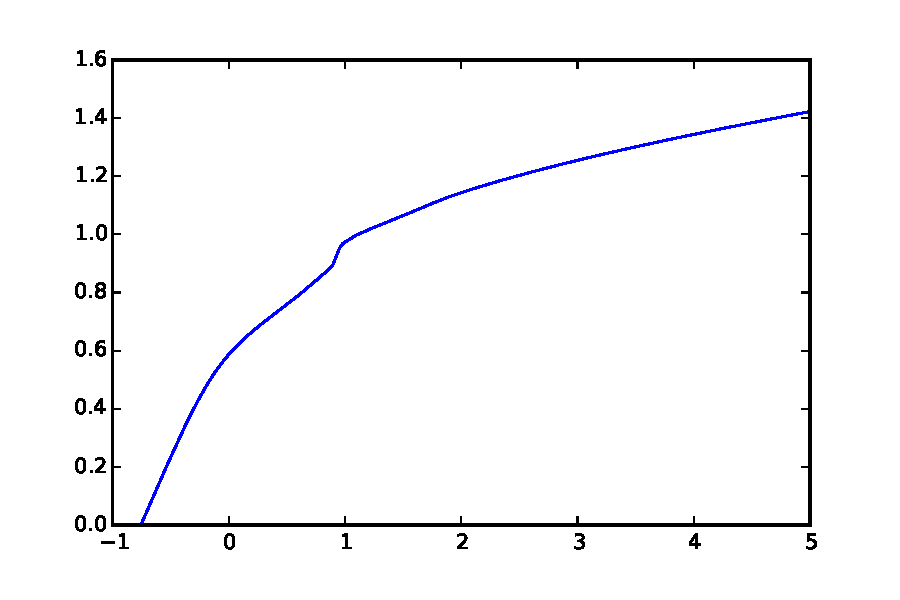
\includegraphics[scale=0.75]{KinkedRcFunc.pdf}
  \end{center}
\end{frame}


% ========== Preference Shocks =================
\begin{frame}
  \frametitle{Marginal Utility Shocks (1/4)}
  Consider another small modification to \texttt{IndShockModel}:
  \bi
\item Multiplicative (idiosyncratic) shocks to utility each period.

\item Consumption ``more valuable'' in some periods than others.
  \ei
  \begin{eqnarray*}
    u(c;\eta) &=& \eta \frac{c^{1-\rho}}{1-\rho}, \qquad \eta_t \sim F_{\eta}, \\
    v(m_t,\eta_t) &=& \max_{c_t} u(c_t;\eta_t) + \beta \PLives_{t+1} \Ex [v_{t+1}(m_{t+1}) ], \\
    a_t &=& m_t - c_t, \qquad a_t \geq \underline{a}, \\
    m_{t+1} &=& R/(\Gamma_{t+1} \psi_{t+1}) a_t + \theta_{t+1}, \\
    \theta_{t+1} \sim F_{\theta t+1}, &\qquad& \psi_{t+1} \sim F_{\psi t+1}, \hspace{0.25cm} \Ex[\psi_{t+1}] = 1.
  \end{eqnarray*}
\end{frame}

\begin{frame}
  \frametitle{Marginal Utility Shocks (2/4)}
  New input \texttt{PrefShkDstn} is constructed:
  \begin{itemize}
  \item \texttt{PrefShkStd}: Standard deviation of (log) pref shocks

  \item \texttt{PrefShkCount}: Number of discrete shocks in ``body''

  \item \texttt{PrefShkTailCount}: Discrete shocks in ``augmented tail''
  \end{itemize}
\end{frame}

\begin{frame}
  \frametitle{Marginal Utility Shocks (3/4)}
  \texttt{ConsPrefShockSolver} inherits from \texttt{ConsIndShockSolver}

  \begin{block}{Additions to \texttt{\_\_init\_\_} method:}
    \begin{itemize}
    \item 2 lines: Store preference shock distribution \texttt{PrefShkDstn}
    \end{itemize}
  \end{block}

  \begin{block}{Replace \texttt{getPointsForInterpolation}}
    \begin{itemize}
    \item 8 lines: Values of $c_t$ and $m_t$ for each $\eta_t$ in \texttt{PrefShkDstn}
    \end{itemize}
  \end{block}

  \begin{block}{Replace \texttt{usePointsForInterpolation}}
    \begin{itemize}
    \item 6 lines: Construct \texttt{cFunc} as a \texttt{LinearInterpOnInterp1D}

    \item 6 lines: Make \texttt{vPfunc} by integrating marginal utility across $\eta_t$
    \end{itemize}
  \end{block}
\end{frame}

\begin{frame}
  \frametitle{Marginal Utility Shocks (4/4)}
  \begin{center}
    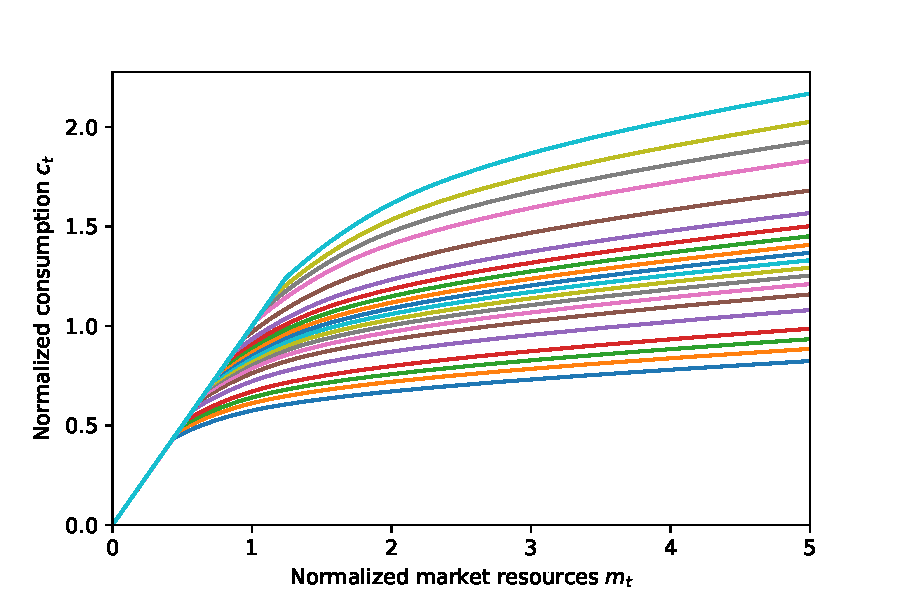
\includegraphics[scale=0.75]{PrefShockcFunc.pdf}
  \end{center}
\end{frame}

% ========== Kinky Preferences =================
\begin{frame}
  \frametitle{Combination Inheritance: ``Kinky Preferences'' (1/4)}
  Combine those two extensions to \texttt{IndShockModel}:
  \begin{itemize}
  \item Borrowing has higher interest rate than saving...

  \item ...and there are shocks to marginal utility

  \item HARK makes this pretty easy
  \end{itemize}
\end{frame}

\begin{frame}
  \frametitle{Combination Inheritance: ``Kinky Preferences'' (2/4)}
  \begin{eqnarray*}
    u(c,\eta) &=& \eta \frac{c^{1-\rho}}{1-\rho}, \qquad \eta_t \sim F_{\eta},\\
    v(m_t,\eta_t) &=& \max_{c_t} u(c_t) + \beta \PLives_{t+1} \Ex [v_{t+1}(m_{t+1}) ], \\
    a_t &=& m_t - c_t, \qquad a_t \geq \underline{a}, \\
    m_{t+1} &=& R/(\Gamma_{t+1} \psi_{t+1}) a_t + \theta_{t+1}, \\
    \theta_{t+1} \sim F_{\theta t+1}, &\qquad& \psi_{t+1} \sim F_{\psi t+1}, \hspace{0.25cm} \Ex[\psi_{t+1}] = 1, \\
    R &=& \begin{cases}
      R_{boro} & \text{if  } a_t < 0 \\
      R_{save} & \text{if  } a_t > 0
    \end{cases}, \qquad R_{boro} \geq R_{save}.
  \end{eqnarray*}
\end{frame}

\begin{frame}
  \frametitle{Combination Inheritance: ``Kinky Preferences'' (3/4)}
  \texttt{ConsKinkyPrefSolver} inherits from two parent classes.  Entirety of the code for the solver:

  \scriptsize{
    \texttt{
      class ConsKinkyPrefSolver(ConsPrefShockSolver,ConsKinkedRsolver):\\
      \qquad def \_\_init\_\_(self,solution\_next,...):\\
      \qquad \qquad ConsKinkedRsolver.\_\_init\_\_(self,solution\_next,...)\\
      \qquad \qquad self.PrefShkPrbs = PrefShkDstn[0]\\
      \qquad \qquad self.PrefShkVals = PrefShkDstn[1]\\
    }}
\end{frame}


\begin{frame}
  \frametitle{Combination Inheritance: ``Kinky Preferences'' (4/4)}
  \hyperlink{DiscussionTopics}{\beamerbutton{Back}}

  \begin{center}
    \includegraphics[scale=0.75]{KinkyPrefcFunc.pdf}
  \end{center}

\end{frame}




% =========== MACROECONOMICS ===========================

\begin{frame}\label{Macroeconomics}
  \frametitle{Macroeconomics in HARK (1/5)}
  \bi
\item <1->Some inputs to micro models are exogenous to each agent...

\item <1->...But endogenous to collective whole of agents

\item <1->Might be static quantities or dynamic processes

\item <2->Equilibrium: consistency between what agents \textit{believe} the endogenous objects are and what values / dynamic processes \textit{actually occur} when agents act on those beliefs

\item <2->Fixed point in the space of beliefs

\item <3->Need a representation of beliefs about endogenous objects

\item <3->And a rule for how agents form beliefs from observing history
  \ei
\end{frame}


\begin{frame}
  \frametitle{Macroeconomics in HARK (2/5)}
  ``The computational algorithm has two key features.  First, it is based on bounded rationality in the sense that we endow agents with boundedly rational perceptions of how the aggregate state evolves...  Second, we use solution by simulation, which works as follows: (i) given the boundedly rational perceptions, we solve the individuals' problems using standard dynamic programming methods; (ii) we draw individual and aggregate shocks over time for a large number of individuals; (iii) ...we generate a time series for all aggregates; and finally (iv) we compare the perceptions about the aggregates to those in the actual simulations, and these perceptions are then updated.  We think this approach... can be productive for other applications.''\\ --Per Krusell and Tony Smith (2006)
\end{frame}



\begin{frame}
  \frametitle{Macroeconomics in HARK (3/5)}
  HARK operationalizes K-S method with a farming metaphor:

  \begin{enumerate}
  \item Solve agents' microeconomic problem for some beliefs

  \item Simulate many agents for many periods by looping on:
    \bi
  \item \texttt{sow}: Distribute current aggregate variables to agents

  \item \texttt{cultivate}: Agents act according to their micro solution

  \item \texttt{reap}: Collect some individual variables from the agents

  \item \texttt{mill}: Generate aggregate variables from individual vars

  \item \texttt{store}: Record some information in a ``history''
    \ei

  \item Use history to update beliefs about endogenous objects
  \end{enumerate}

  \texttt{Market}'s method \texttt{solve} loops on this process until convergence.
\end{frame}


\begin{frame}
  \frametitle{Macroeconomics in HARK (4/5)}
  Attributes of a \texttt{Market} instance (or subclass):
  \bi
\item <1->\texttt{agents}: List of \texttt{AgentType} instances in market

\item <1->\texttt{dyn\_vars}: Names of the endogenous objects

\item <2->\texttt{sow\_vars}: Names of aggregate variables

\item <2->\texttt{reap\_vars}: Individual variables that form aggregates

\item <2->\texttt{track\_vars}: Aggregates that need to be recorded in history

\item <3->\texttt{millRule}: Function that transforms ind $\longrightarrow$ agg variables

\item <3->\texttt{calcDynamics}: Function that transforms history into beliefs
  \ei
\end{frame}



\begin{frame}
  \frametitle{Macroeconomics in HARK (5/5)}
  Extra methods of a \texttt{Market}-compatible \texttt{AgentType}:
  \bi
\item \texttt{marketAction}: What agents \textit{do} to generate \texttt{reap\_vars}.  Often just simulate one period with \texttt{simOnePeriod}

\item \texttt{reset}: How to initialize for a new history: reset states
  \ei

  Trivial to add more \textit{ex ante} heterogeneity: just add more \texttt{AgentType} instances to \texttt{agents}!
\end{frame}



% ============ Agg shocks model ====================
\begin{frame}
  \frametitle{Consumption-Saving with Aggregate Productivity Shocks}
  \begin{eqnarray*}
    v_t(m_t,M_t) &=& \max_{c_t} u(c_t) + \beta \PLives_{t+1} \Ex [v_{t+1}(m_{t+1},M_{t+1}) ], \\
    a_t &=& m_t - c_t, \qquad a_t \geq 0, \\
    m_{t+1} &=& \frac{R_{t+1} a_t}{\Gamma_{t+1}\psi_{t+1} \Psi_{t+1}}  + W_{t+1} \theta_{t+1} \Theta_{t+1} \ell, \\
    A_t = \textbf{A}({M_t}),  & & k_{t+1} = (1-\delta)A_t/(\Psi_{t+1} \ell), \\
    R_{t+1} = \textbf{R}(k_{t+1}/\Theta_{t+1}), & & W_{t+1} = \textbf{W}(k_{t+1}/\Theta_{t+1}), \\
    M_{t+1} &=& R_{t+1} k_{t+1} + W_{t+1} \Theta_{t+1} \ell \\
    \theta_{t+1} \sim F_{\theta t+1}, &\qquad& \psi_{t+1} \sim F_{\psi t+1}, \hspace{0.25cm} \Ex[\psi_{t+1}] = 1, \\
    \Theta_{t+1} \sim F_{\Theta}, &\qquad& \Psi_{t+1} \sim F_{\Psi}, \hspace{0.25cm} \Ex[\Psi_{t+1}] = \Ex[\Theta_{t+1}] = 1.
  \end{eqnarray*}
\end{frame}



\begin{frame}
  \frametitle{Consumption-Saving with Aggregate Productivity Shocks}
  Some totally new inputs for an \texttt{AggShockConsumerType}:
  \begin{itemize}
  \item \texttt{Rfunc} and \texttt{wFunc}: Factor payments as function of $k_t$

  \item \texttt{Mgrid}: Grid of $M_t$ state values (sort of constructed)

  \item \texttt{Afunc}: $\Ex[A_t | M_t] = \mathbf{A}(M_t)$
  \end{itemize}

  \texttt{IncomeDstn} combines idiosyncratic and aggregate shocks:
  \begin{itemize}
  \item Discrete approximation to aggregate shock distribution constructed like idiosyncratic shocks: \texttt{PermShkAggStd}, \texttt{TranShkAggStd}, \texttt{PermShkAggCount}, \texttt{TranShkAggCount}

  \item \texttt{IncomeDstn} has five elements: probs, idio shocks, agg shocks
  \end{itemize}
\end{frame}

\begin{frame}
  \frametitle{Consumption-Saving with Aggregate Productivity Shocks}
  \begin{center}
    \includegraphics[scale=0.75]{AggShockcFunc.pdf}
  \end{center}
\end{frame}



\begin{frame}
  \frametitle{Cobb-Douglas Economy in the \texttt{Market} Framework}

  \texttt{CobbDouglasEconomy} is a subclass of \texttt{Market}:

  \bi
\item \texttt{sow}: Distribute $(M_t,R_t,W_t,\Theta_t,\Psi_t)$ to consumers

\item \texttt{cultivate}: Consumers draw $(\theta_t,\psi_t)$, choose $c_t$

\item \texttt{reap}: Collect assets $a_t$ and productivity $P_t$ from consumers

\item \texttt{mill}: Calc $A_{t+1}$, draw $(\Theta_{t+1},\Psi_{t+1})$, calc $k_{t+1}, M_{t+1}$, get $(R_{t+1},W_{t+1})$

\item \texttt{store}: Record $M_t$ and $A_t$ in their histories
  \ei

  Loop that process for (say) 1000 periods
  \begin{itemize}
  \item \texttt{calcDynamics}: Regress $log(A_t)$ on $log(M_t)$, make new \textbf{A}

  \item Distribute new \textbf{A} to consumers as \texttt{Afunc}
  \end{itemize}
\end{frame}



\begin{frame}
  \frametitle{Other Applications of \texttt{Market}}
  Krusell and Smith were right: method is applicable to other topics

  \bi
\item <1->Premiums of medical insurance contracts: actuarial constraint maps \textit{who} buys each contract to break even premium, subject to informational constraints (sex, age, health, etc)

\item <2->Papageorge et al risky sex framework: probability of contracting HIV from risky sex act depends on HIV infection rate and risky sex choices of the population

\item <3->Agent-to-agent interaction: could \texttt{sow} a permutation of what is \texttt{reap}ed: imperfect knowledge, contagion of information, moves closer to ``agent-based modeling''
  \ei

  \hyperlink{DiscussionTopics}{\beamerbutton{Back}}

\end{frame}

\beamerdefaultoverlayspecification{<*>}

\begin{frame}[t,allowframebreaks]
  \frametitle{References}
  \tiny 
  \input econtexBibMake
\end{frame}
\pagebreak

\end{document}